\subsection{Factory Method}

\subsubsection*{Problembeschreibung}

Es wird eine Schnittstelle benötigt, um eine Reihe von Objekten erzeugen zu können. Jedes Objekt hat jedoch andere Anforderungen an seine Erzeugung. Eine \emph{Factory-Method} kann eingesetzt werden, wenn eine Klasse kein Wissen darüber besitzt oder besitzen soll, welches konkrete Objekt sie zu erzeugen hat oder wenn eine Klasse die Verantwortlichkeit über diese Entscheidung ihren Subklassen überlassen soll. \cite{gamma_design_1995}

\subsubsection*{Lösung}

Es existiert ein abstrakter Erzeuger (\code{Creator}), welcher eine Schnittstelle bereitstellt, um Produkte (\code{Product}) zu erzeugen. Die Details der Erzeugung dieser Produkte sind in den konkreten Subklassen der Erzeuger-Klasse implementiert. Jeder konkrete Erzeuger kann somit einen Typ von konkretem Produkt (\code{ConcreteProduct}) erschaffen. Das entsprechende Klassendiagramm ist in \autoref{fig:factory-method-class} dargestellt.

\begin{figure}[!ht]
	\centering
	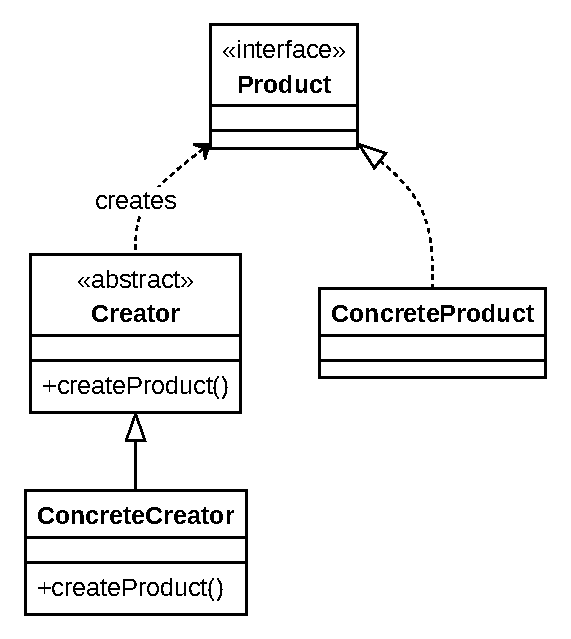
\includegraphics[width=0.75\linewidth]{images/patterns/factory-method-class.pdf}
	\caption{Klassendiagramm des \emph{Factory-Method}-Musters. Für jedes konkrete Produkt existiert ein konkreter \emph{Creator}, welcher eine \emph{Factory Method} \code{createProduct} besitzt. Diese erzeugt das korrespondierende Produkt. Dabei spiegelt die Vererbungshierarchie der \emph{Creator} die der Produkte. \cite{skobeleva_factory_2023}}
	\label{fig:factory-method-class}
\end{figure}

\subsubsection*{Konsequenzen}
Ein Objekt über eine \emph{Factory-Method} zu erzeugen ist flexibler, als das Objekt direkt über den Konstruktor der Klasse zu instanziieren. Die erzeugende Klasse braucht nur das Interface des abstrakten Erzeugers zu kennen und ist somit in der Lage beliebige konkrete Produkte über deren korrespondierende konkrete Erzeuger zu instanziieren. Hierbei fällt auf, dass die Erzeuger-Klassenhierarchie die Produkt-Klassenhierarchie spiegelt. Für jeden Produkttyp existiert also auch eine Erzeuger-Klasse. Daraus kann sich jedoch auch ein Nachteil ergeben. Zur Nutzung eines Produktes müssen nun stets zwei Subklassen definiert und zur Laufzeit ein weiteres Objekt erstellt werden. Das erhöht die Komplexität. \cite{gamma_design_1995}

